\section[Field Monitoring]{Field Monitoring
\footnote{
  $CVS~revision~ $Id: nmr-1999.tex,v 1.4 2003/12/17 03:59:48 gen Exp $ $ 
}
\footnote{Authors: J.LeRose \email{lerose@jlab.org}}
}

The field-monitoring controls are available using the main 
HRS screen%
\infolevtwo{ (see Figure~\ref{fig:hrs_mag_cntrl})%
}. % infolev
The dipoles' field is measured using NMR Teslameters and
field probes.

\infolevone{ 
 
\subsection{ Dipole Field Monitoring Electron Arm}

\noindent {\bf Basic Setup}

Each spectrometer dipole magnet is equipped with a Metrolab PT 4025 
NMR Teslameter, several field probes, and multiplexers (to allow switching 
between the probes).  Details of the operation and theory of operation 
for the Teslameter can be found in its user manual, 
a copy of which is available in the the counting house.
The basic layout is shown in Figure~\ref{fig:nmrbasic}


\begin{figure}
\begin{center}
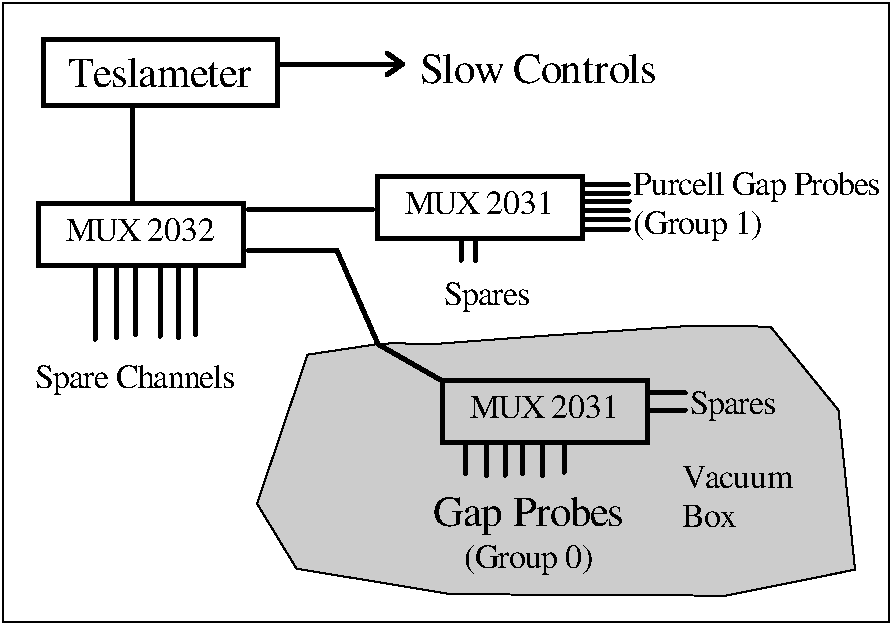
\includegraphics[angle=0,width=15cm,clip]{lerose_fig1}
{\linespread{1.}
\caption[Spectrometers: NMR System Layout]{Basic layout of NMR system}
\label{fig:nmrbasic}}
\end{center}
\end{figure}


 The "Gap Probes" (Group 0 in the controls) are located in two groups 
of three; one group on the low field side of the gap and the other on the high 
field side of the gap.  The groups of three are made up of one each of 
the manufacturer's type 3, 4 \& 5 probes, designed to cover different 
field ranges (see Table \ref{nmr_range}).  The six ``Purcell Gap Probes'' (Group 1 in 
the controls) are located in the Purcell gap of the magnet 
and consists of two each of the above types. {\em Note: Since
the fall of 1998 the multiplexer-multiplexer in both arms,
MUX 2032, has been removed and hence the ``Purcell Gap Probes'' are currently
unavailable. There are no plans to re-install this multiplexer.}

 The "Gap Probes" are equipped with coils which provide a field 
gradient that cancels out the field gradient of the magnet in the vicinity of 
the probe.  These gradient compensating coils are part of a simple circuit 
that is completely independent of the Teslameter.  The basic circuit for 
the compensating coils is shown in Figure~\ref{fig:nmrcir}


\begin{figure}
\begin{center}
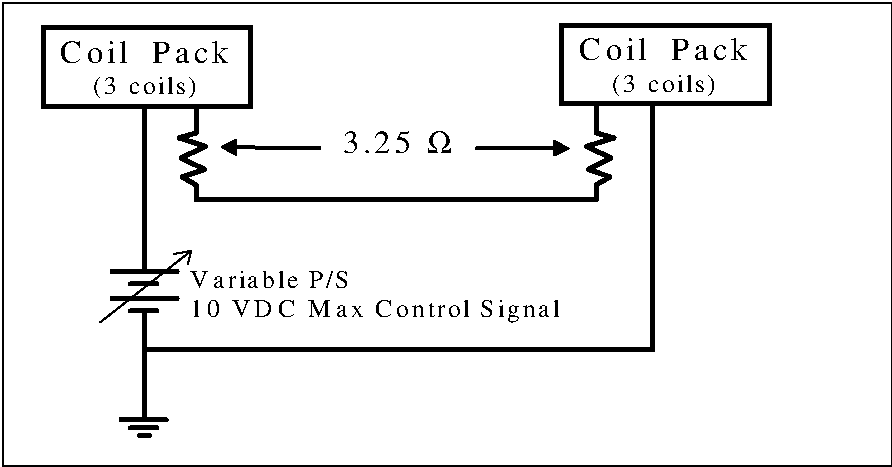
\includegraphics[angle=0,width=10cm,clip]{lerose_fig2}
{\linespread{1.}
\caption[Spectrometers: NMR Gradient Compensation]{Gradient Compensating Circuit.}
\label{fig:nmrcir}}
\end{center}
\end{figure}


%\snfig{figs/lerose_figcce.eps}{Control Voltage calibration for
%Electron Dipole }{nmrcomp4}{5in}

\begin{figure}
\begin{center}
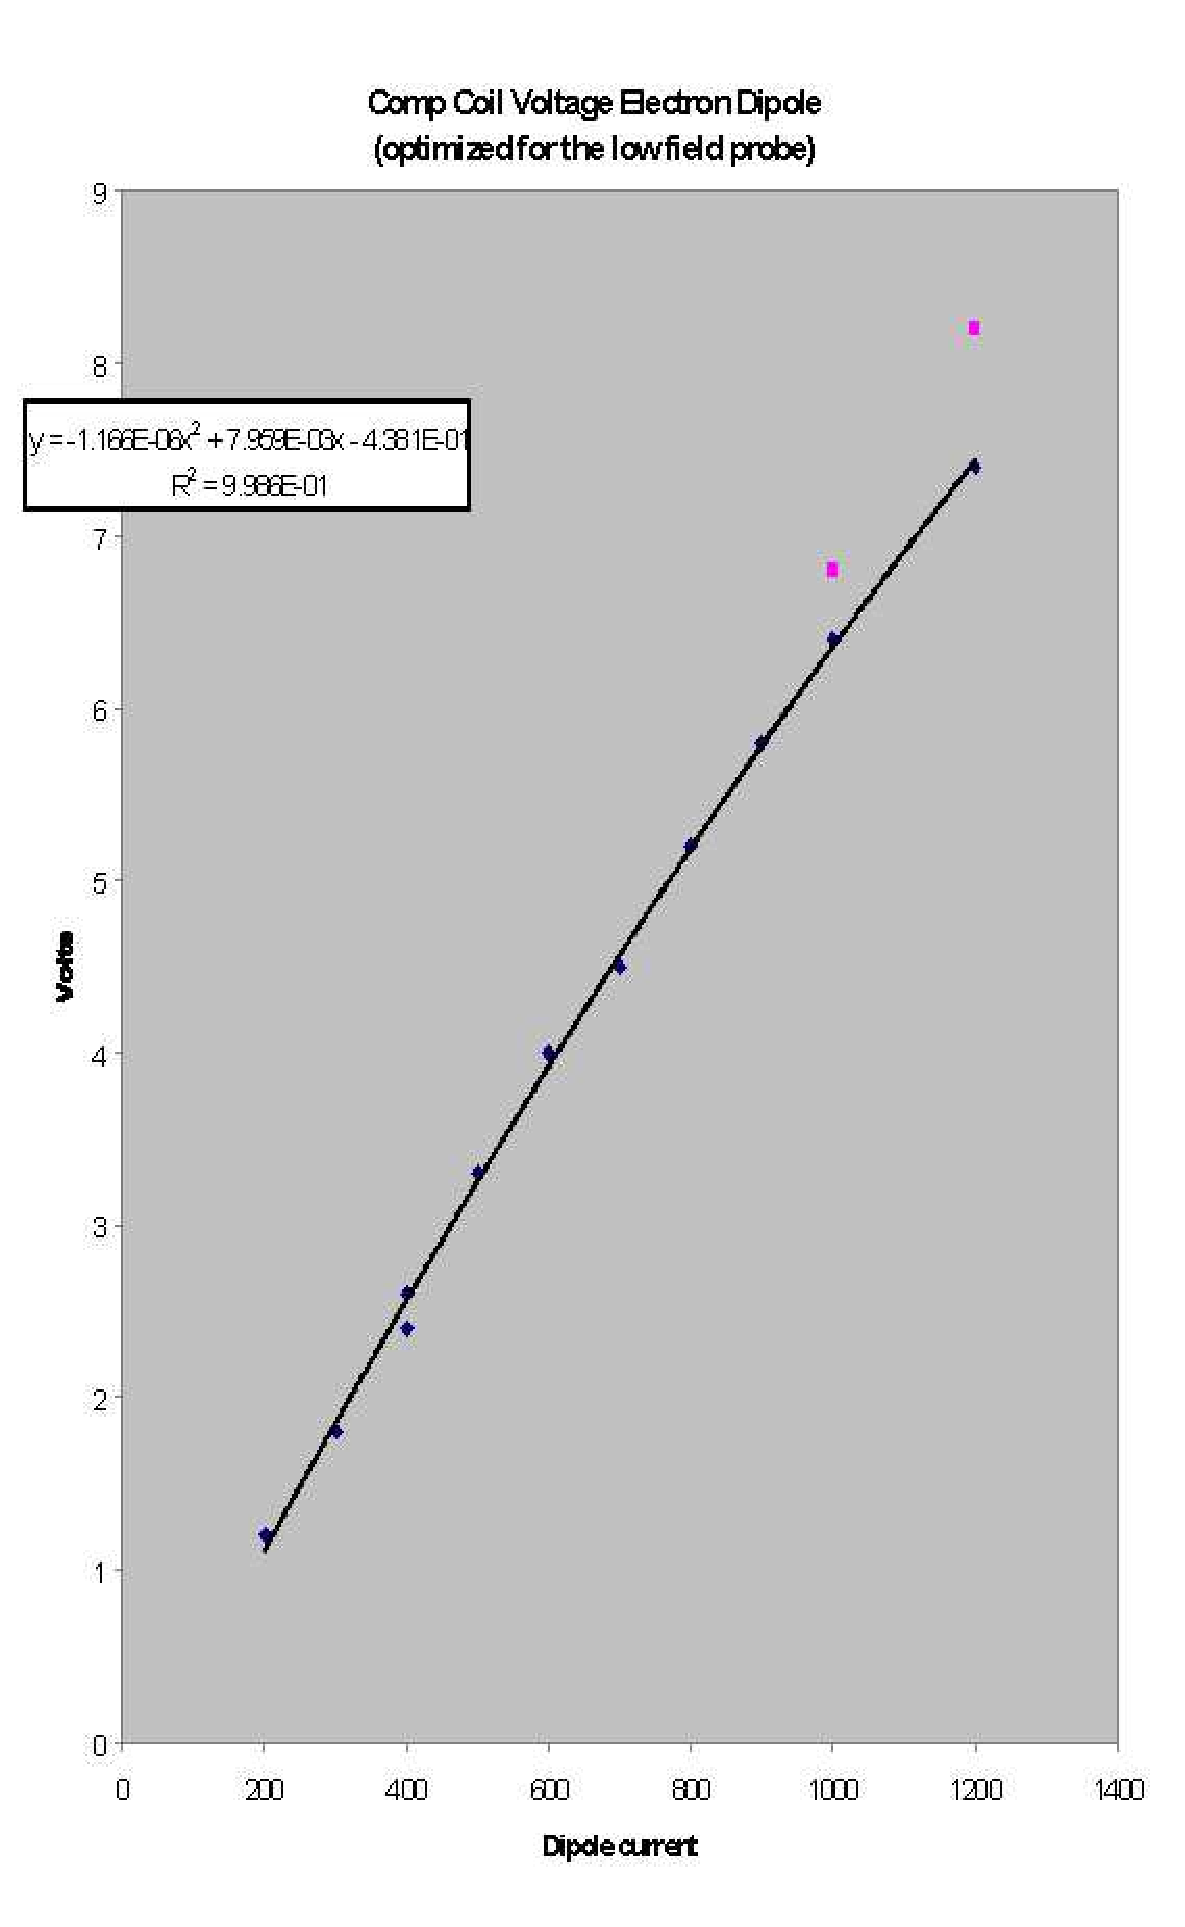
\includegraphics[angle=0,height=20cm,clip]{lerose_figcce}
{\linespread{1.}
\caption[Spectrometers: Control Voltage Calibration for Left Dipole]{Control Voltage calibration for the Left Dipole.}
\label{fig:nmrcomp4}}
\end{center}
\end{figure}

%\snfig{figs/lerose_figcch.eps}{Control Voltage calibration for
%Hadron Dipole }{nmrcomp5}{5in}
\begin{figure}
\begin{center}
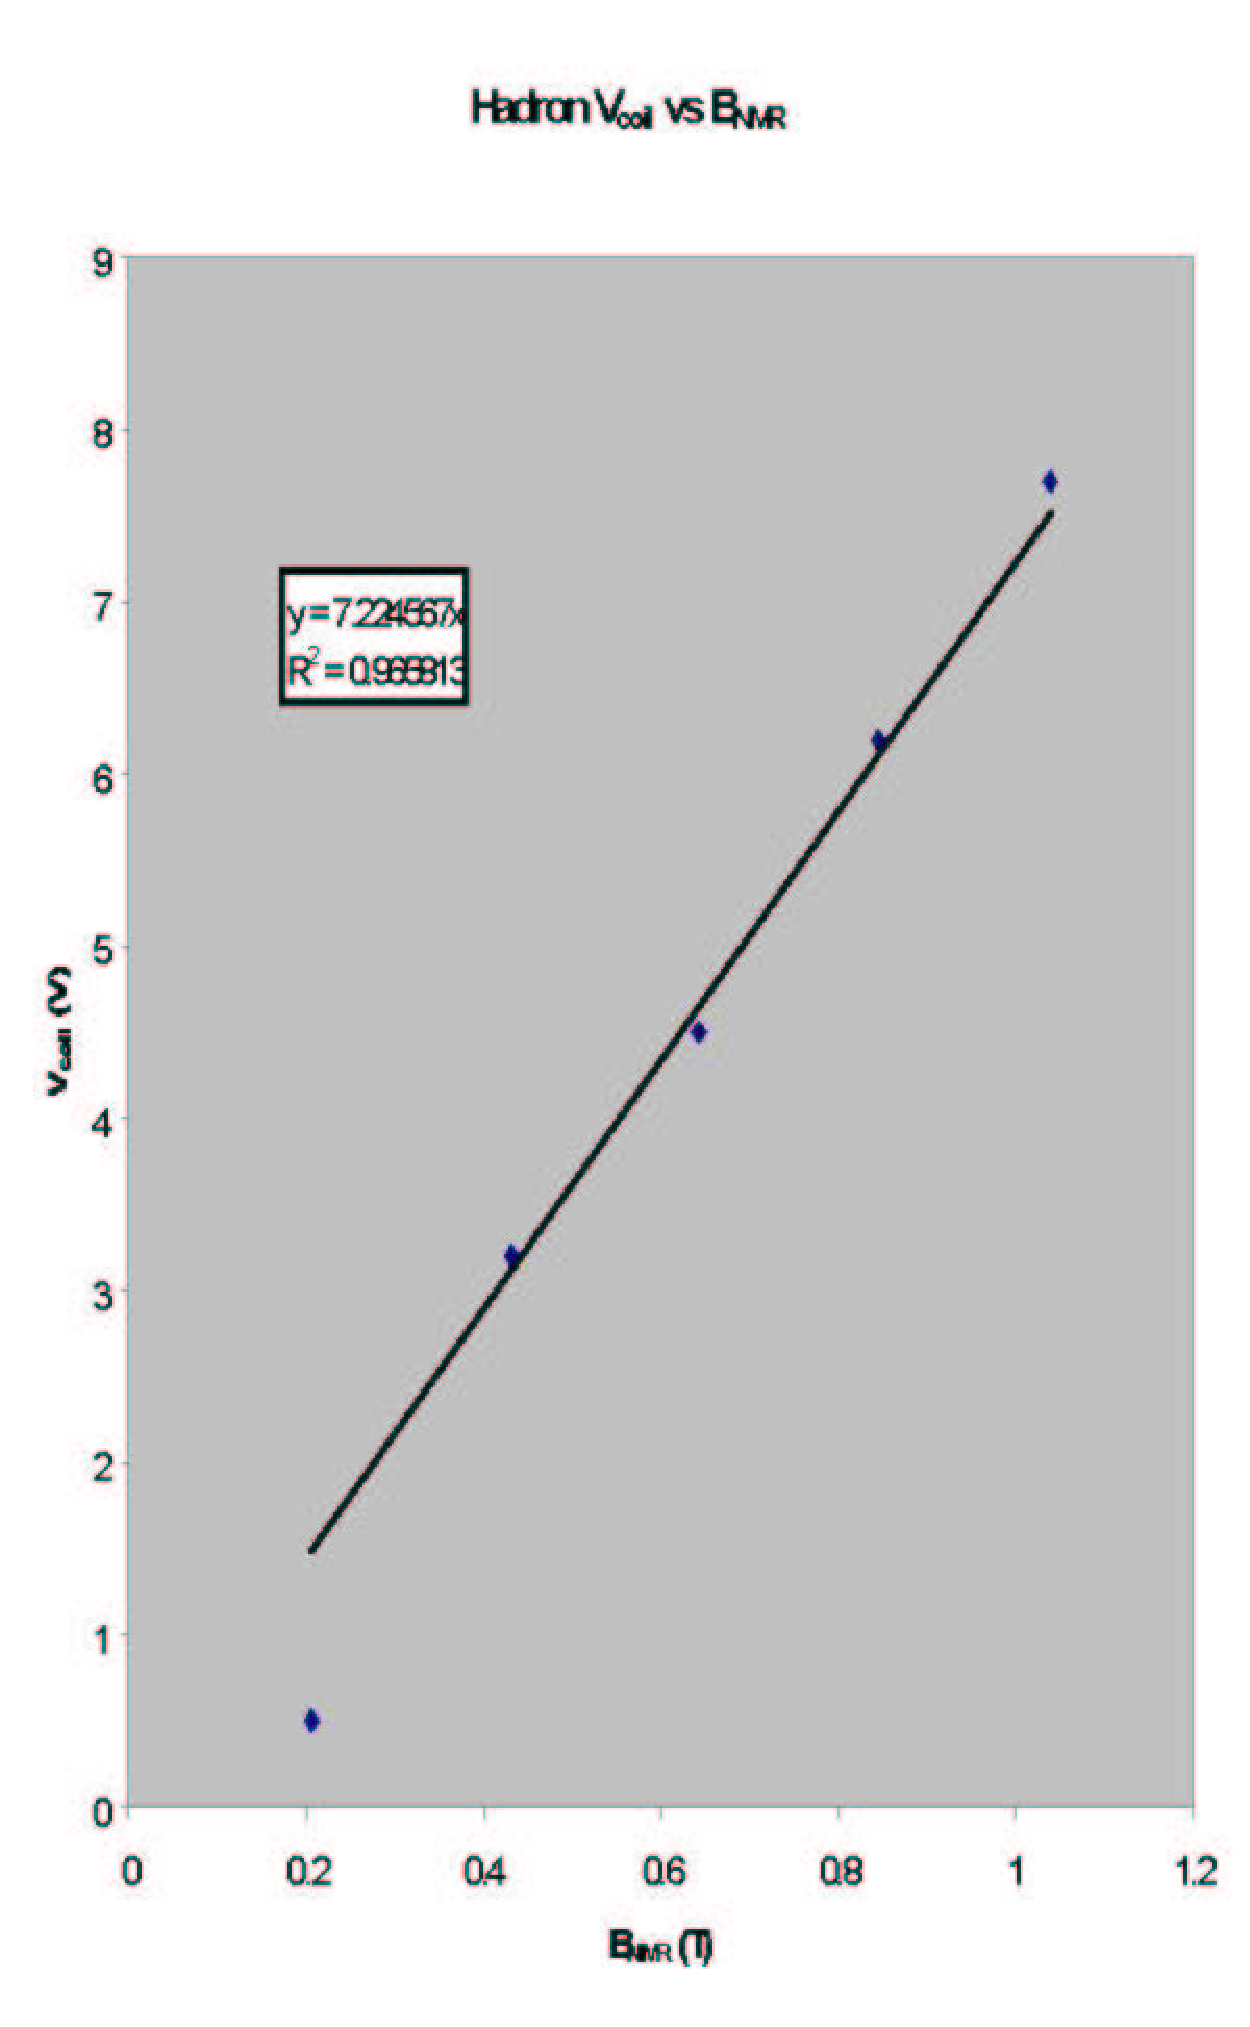
\includegraphics[angle=0,height=20cm,clip]{lerose_figcch}
{\linespread{1.}
\caption[Spectrometers: Control Voltage Calibration for Right Dipole] {Control Voltage calibration for the Right Dipole.}
\label{fig:nmrcomp5}}
\end{center}
\end{figure}

%\snfig{./figs/lerose_fig7.eps}{DAC Calibration for manual operation of NMR probes}{nmr_dac}{9in}
\begin{figure}
\begin{center}
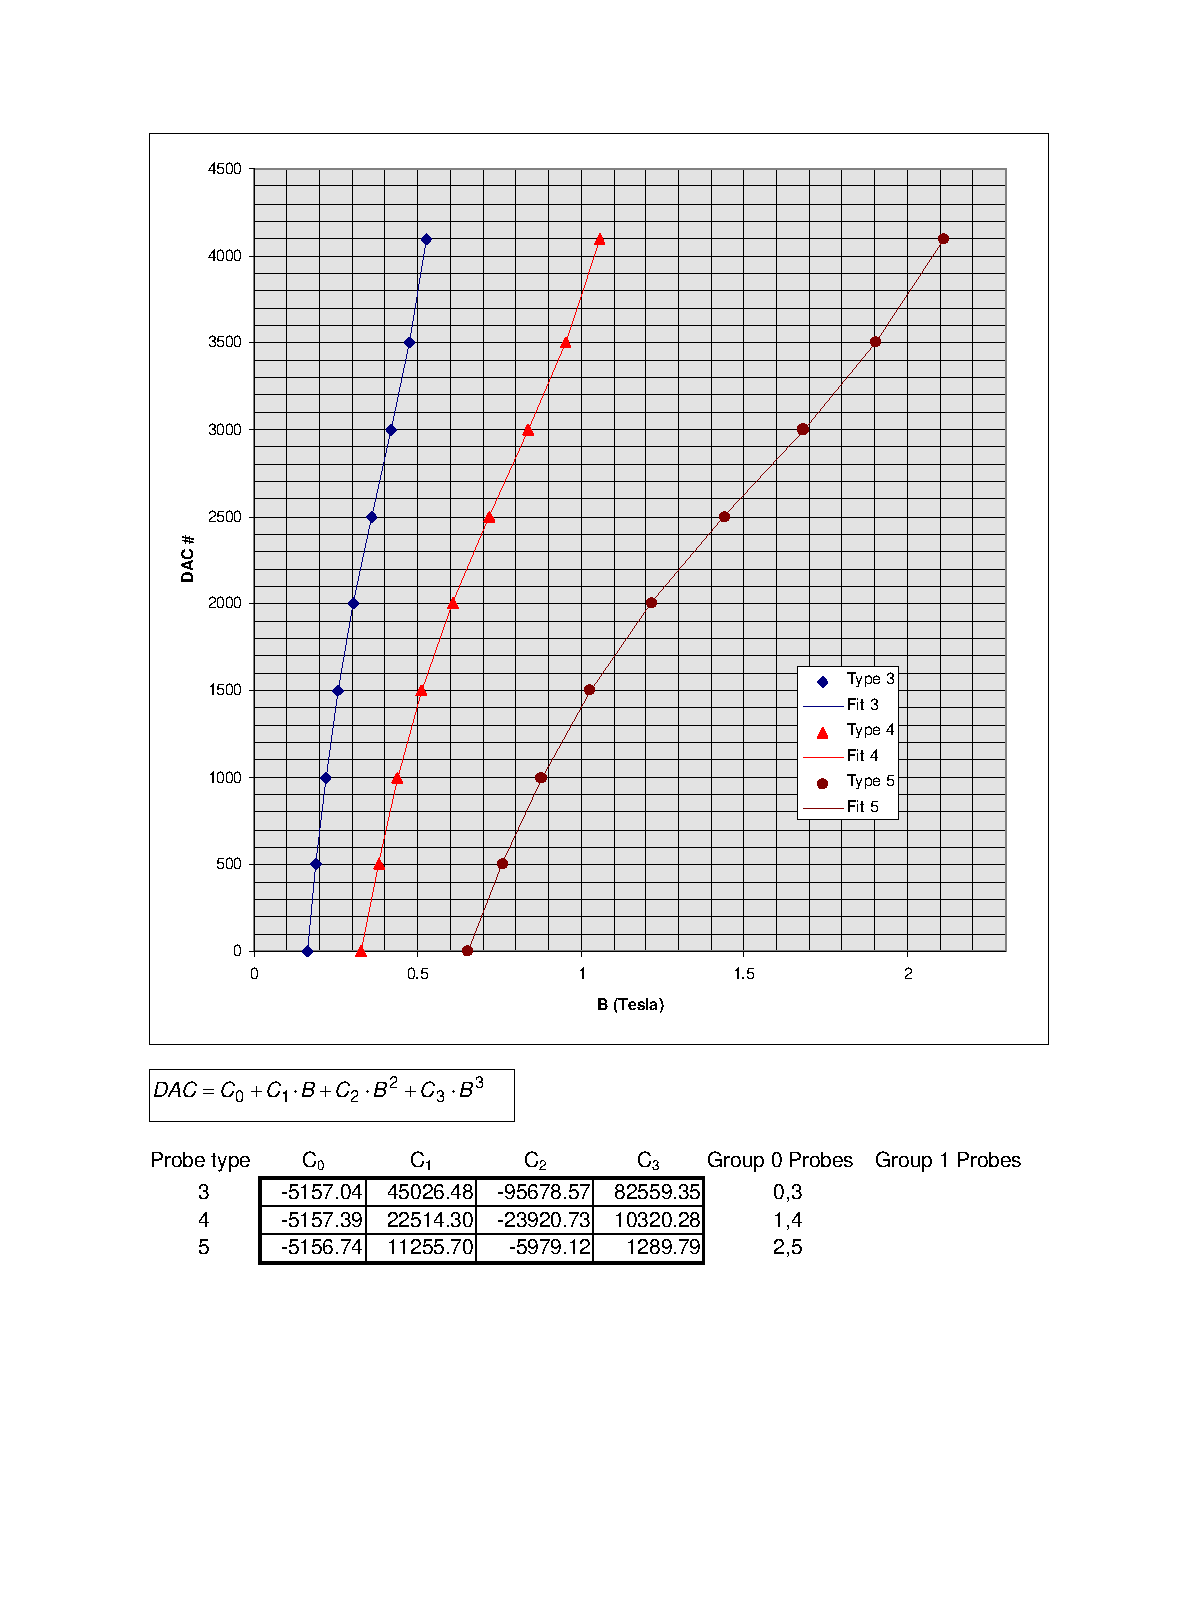
\includegraphics[angle=0,height=20cm,clip]{lerose_fig7}
{\linespread{1.}
\caption[Spectrometers: NMR Probe DAC Calibration]{DAC Calibration for manual operation of NMR probes.}
\label{fig:nmr_dac}}
\end{center}
\end{figure}

The following graphs (see Figures~\ref{fig:nmrcomp4} 
and ~\ref{fig:nmrcomp5}),can be used to determine optimum values for the 
compensating coil control voltage.  It should be noted that the setting 
of the compensating coil current is not very critical in most cases.  In 
general if you're within 10\% of the correct value everything should 
work fine.



\begin{table}
\begin{center}
\begin{tabular}{|cc|} \hline
Probe Type & Field Range (T) \\ \hline 
3 & 0.17 - 0.52 \\
4 & 0.35 - 1.05 \\
5 & 0.70 - 2.10 \\ \hline
\end{tabular}
\caption[Spectrometers: Dipole NMR Probe Field Ranges]{Dipole NMR probe field ranges}
\label{nmr_range}
\end{center}
\end{table}

} %infolev

\infolevtwo{
\subsection{NMR Operating Procedure}

When running in Autopilot mode (see: Simple Spectrometer Field Setting) the 
compensating coil voltage is set automatically and the probe appropriate for 
the field desired is selected. The gaussmeter is placed in SEARCH Mode and the 
dipole power supply software regulator is turned on. In this case the dipole current is 
adjusted to achieve the desired field. The user should just stand 
back and let it work. What follows are instructions for using
the NMR gaussmeter in situations where Autopilot doesn't work or
some special supplemental measurements are required. 

 In principle it is possible to make the field measurements using the 
SEARCH mode in the Teslameter.  In this mode you select a probe and the 
meter explores the whole field range of the probe until it finds and 
"locks" on the resonant signal indicating that it has a field 
measurement.  A ``lock" is indicated on the controls display by an ``L'' to 
the left of the field values.  This has the advantage of simplicity but in practice can 
be time consuming and doesn't always work.  The problem being, in 
situations where there is a lot of noise mixed in with the signal, the 
circuitry has problems distinguishing the signal from the noise and gets 
lost before it ever finds a lock.  The problem is exacerbated when the 
field being measured is at the high end of the probe's range.  In this 
case the search starts at the low end and keeps getting hung up on the 
noise and never gets to the field range of interest.  The solution to 
this problem is to tell the device approximately what field it's looking 
for and use the AUTO mode to find the lock.  In the procedure below that 
is what we will be doing.

In any case, for ``gap probes" (group 0) you must energize and adjust 
the gradient compensating coils for the field ranges to be measured before 
trying to make a measurement.

For studies involving 
10\% changes in the field settings the compensating coil current can be 
set once and left alone.


\noindent\underline{\bf Recommended Procedure:}(turn the {\bf SOFTWARE REGULATOR OFF} for all 
non-autopilot field measurements)\\
For group 0 probes set compensating coils appropriately (see figures).\\
Put the meter in MANUAL mode with SEARCH OFF \\
Select a probe \underline{\bf and} polarity (\underline{\bf Group 0:  
Probes 0, 1, 2 negative; Probes 3, 4, 5 positive}) \\
Type in the appropriate DAC number for the field range being measured (see below) \\
Select AUTO and wait for a lock (indicating a valid field reading) \\
Verify that you have a good lock by checking the oscilloscope for a 
clear resonant signal. \\
If you have problems see the table listing problems and possible 
solutions.

\noindent\underline{\bf Selecting DAC Number}

In selecting the DAC number to use for the field of interest use 
either the graph in Figure~\ref{fig:nmr_dac} or the polynomial at the bottom of the same figure.

\pagebreak
\noindent{\bf Problems and Solutions}\\
\begin{table}[htb]
\begin{tabular}{|p{0.4\textwidth}|p{0.55\textwidth}|}\hline
Symptom & Diagnosis and Cure \\ \hline\hline
Weird numbers on displays, controls for all magnets fouled up 
& Need to reboot.  See instructions below. \\ \hline
NMR Teslameter does not respond to commands and display shows all zeros. 
& Meter's communications are somehow hung up. Push {\bf RESET}. \\ \hline
%Will not lock & Very high noise level makes resonance hard to find. \\
%Still 
Will not lock 
& Very high noise level makes resonance hard to find. Search for the resonance manually by 
  adjusting the DAC in manual mode until you see the resonant signal.  (It helps if you know 
  what field you expect so you'll know where to look). \\ \hline
You find resonance manually but still can't get a lock 
& Check probe polarity. Try decreasing and increasing DAC number by 1. Optimize signal 
  by adjusting compensating coils. \\ \hline
Can't find resonance manually 
& Try a different probe.  Use readings from other probes to tell you where to look for 
 the resonance with the probe that's giving you trouble.  Make sure
 compensating coils are energized properly.  Make sure magnet is on. \\ \hline\hline
\end{tabular}
\caption[NMR: Problems and solutions]{NMR: Problems and solutions}
\label{tab:nmr-problems-solutions}
\end{table}

\begin{table}[ht]
\begin{center}
\begin{tabular}{|p{0.3\textwidth}|p{0.3\textwidth}|p{0.3\textwidth}|}\hline
Problems & Explanation & Action \\ \hline
NMR not locked but current is changing in the right direction 
& Normal operation for large field changes  
& Wait. (see above) \\ \hline
NMR locked but current going in the wrong direction.
& Normal operation. 
& Wait. \\ \hline
NMR locked but field not correct and current not changing 
& Field regulation is disabled or software is confused.
& Check that field regulation is enabled. Enter desired field value or one
  very near the desired value again. \\ \hline
NMR field display freezes. (Usually but not always shows  -\#.0000000)
& NMR Gaussmeter is not communicating with software.
& Push {\bf RESET}. \\ \hline
\end{tabular}
\end{center}
\caption[NMR troubleshooting]{NMR troubleshooting
}
\label{tab:hrs_nmr_2}
\end{table}

} %infolev

\begin{safetyen}{10}{15}
\subsection{Authorized Personnel}
\end{safetyen}

The individuals shown in Table \ref{tab:nmr:personnel} are responsible for NMR operation problems.

\begin{namestab}{tab:nmr:personnel}{NMR: authorized personnel}{%
      NMR: authorized personnel.}
  \JackSegal{\em Contact}
\end{namestab}


